\documentclass{school-22.211-notes}
\date{February 27, 2012}

\begin{document}
\maketitle

\topic{Energy Self-Shielding Effects}
As we increase the U/H ratio, the RI decreases in the three big resonance regions, and we see big dips on the spectrum plot. When U/H = 1.0, the spectrum is distorted. There are so much U238 in the fuel, that there is no flux in the fuel anymore. As we increase the number of uranium atoms by a factor of 10, the number of absorption per atom is decreased by a factor of 3. That is, the total aborption still increases, but the absorption per atom decreases. 

Insert slide 26 here. 

\topic{Spectral Hardening}
\textit{As more absorber (uranium in this case) is added, the higher energy ranges become more important, as can be seen that the fraction of absorption happening in the higher energies increase, and the peak of the thermal spectrum shifts to the right as well. The 1/E shape becomes more important as well.}

Insert slide 28. 

\topic{Reactor Type Spectral Optimizations and Sensitivities}




\lecture{Rsonance Absorption}
\topic{Homogenous Resonance Absorption}


\topic{Background Cross Section}


%%%%%%%%%%%%%%%%%%%%%%%%% Qualify Exam Start %%%%%%%%%%%%%%%%%%%%%%%%%%%%
\lecture{Facts For Qualify Exam}
\begin{enumerate}
\item Flux = $\frac{n}{\cm^2 \s}.$

\item Fast flux in hydrogen is around $10^{14}$ n/cm$^2$s, and on the order of $10^{12}$n/cm$^2$s for thermal flux. 

\item Capture cross-section as in Figure~\ref{capture-xs}: 
\begin{figure}
  \centering
  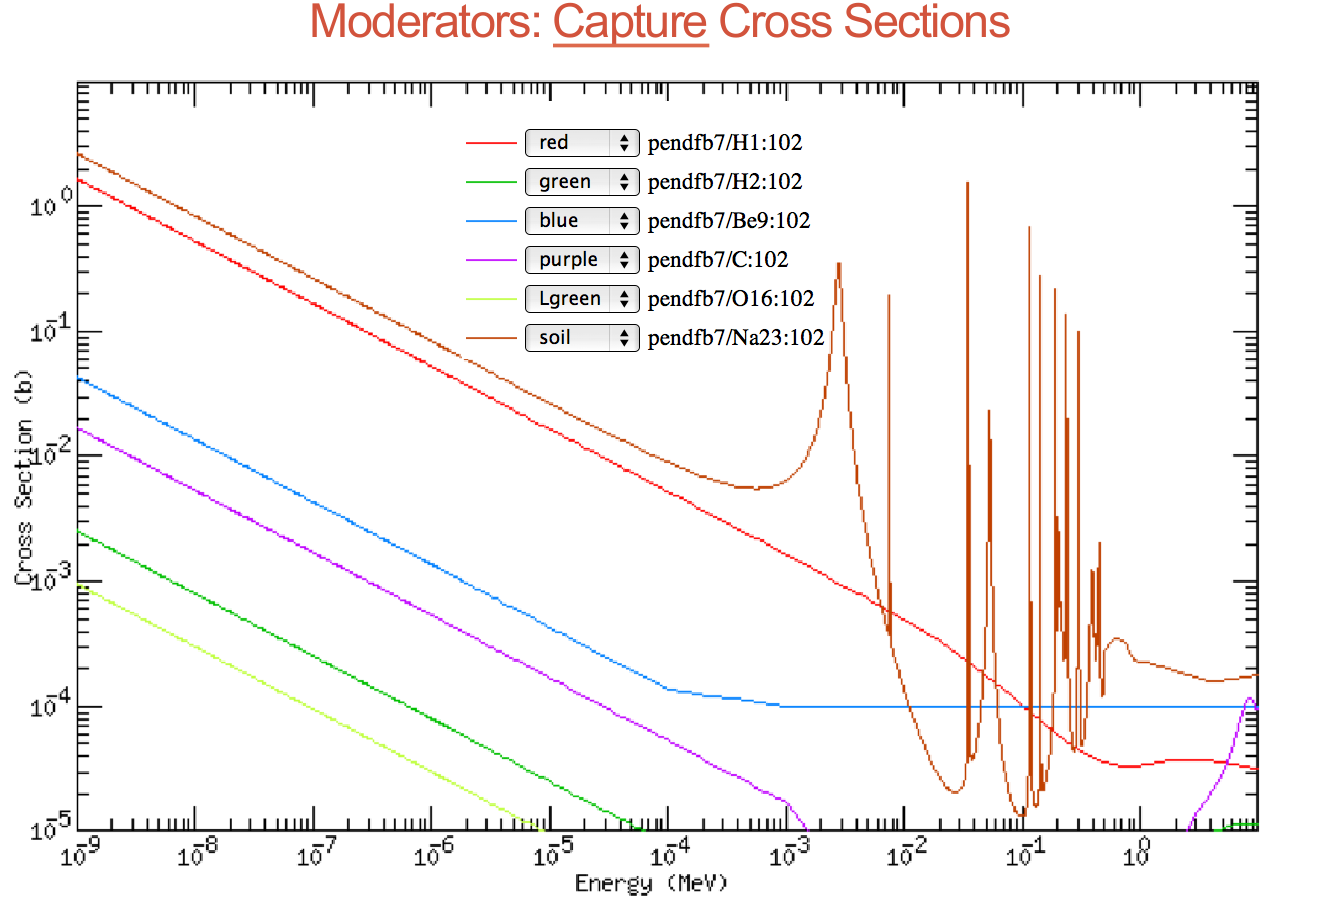
\includegraphics[width=4in]{images/capture-xs.png}
  \\
  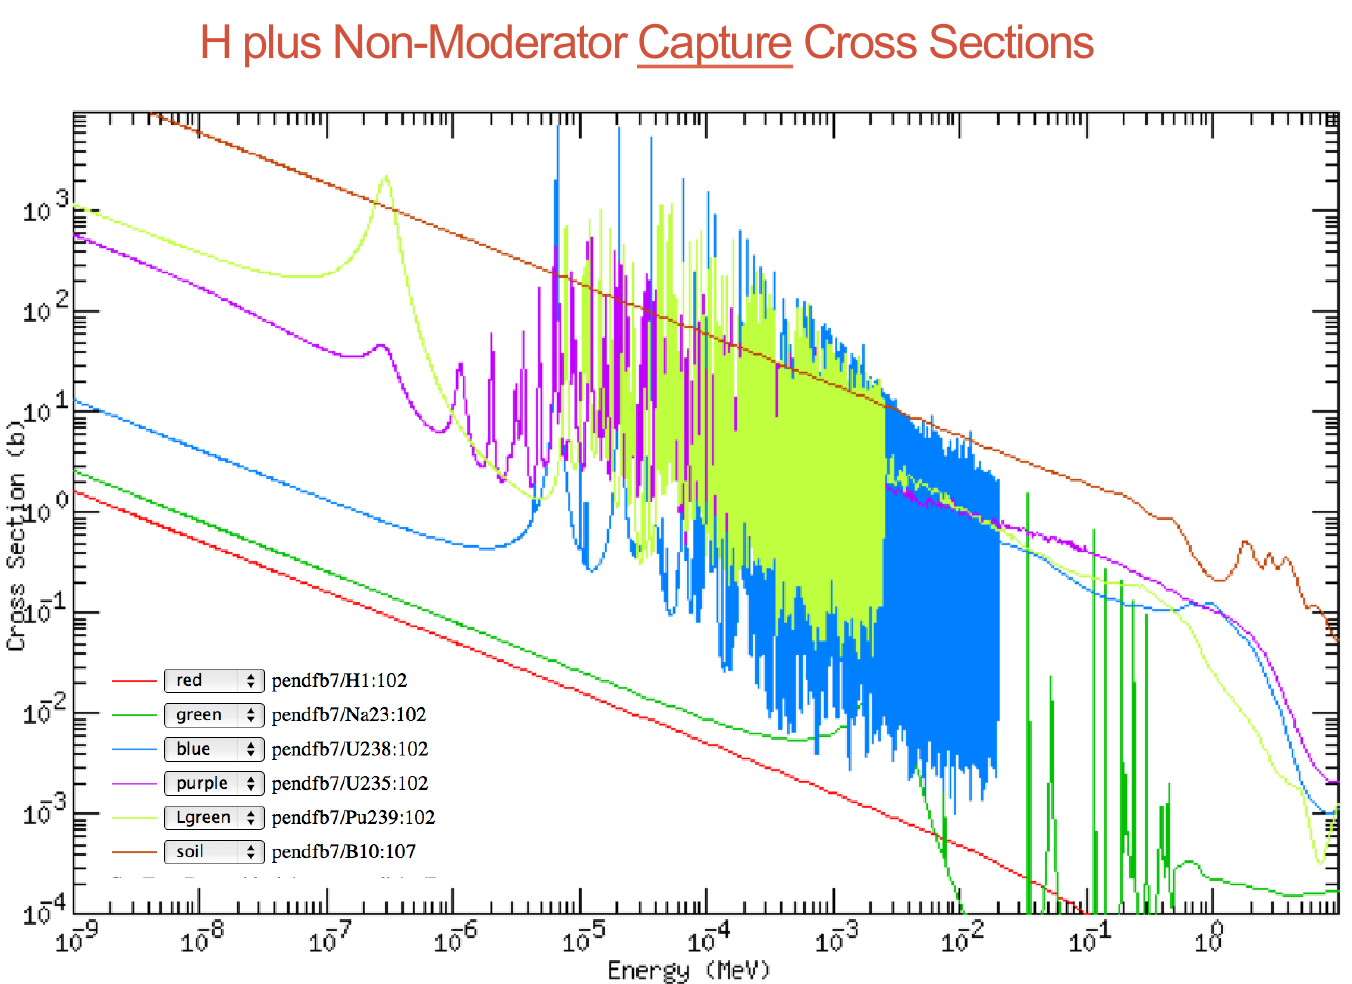
\includegraphics[width=4in]{images/capture-xs-2.png}
  \caption{Capture Cross Section} \label{capture-xs}
\end{figure}
\begin{enumerate}
\item H has no resonance; it has the highest scattering xs in LWR, so we can ignore any other isotopic's neutron scattering.   
\item Na has a huge resonance in 23 keV, and more resonances at higher energies because it is a heavy isotope.
\item Near zero energy,
\eqn{ \sigma(E\to 0) = }
\item Resonance at 6 to 7 eV: U238. 
\item U235's thermal elastic xs is larger than 238's, and they both have resonance around the same range.   
\item A small resonance at .3 eV: Pu239 (its signiture is a super low energy scattering xs). 
\end{enumerate}

\item Given an unknown material type, all we care is to count the nucleus density of each material and look at it's xs. 
\item Average fission neutron energy: 2 MeV; average peak fission energy: 1 MeV; see fission sepctrum. 
\end{enumerate}
%%%%%%%%%%%%%%%%%%%%%%%%% Qualify Exam End %%%%%%%%%%%%%%%%%%%%%%%%%%%%


\end{document}
